\section{Règles de changement d'états et moteur du jeu}

\subsection{Changements extérieurs}
Parmi les changements extérieurs, nous allons créer une "Touche A" pour annuler et revenir au début du tour. Le joueur pourra utiliser cette touche, avant d'avoir lancé les dés, s'il veut finalement choisir d'attaquer un autre pays. % a reflechir, peut-etre difficile -- ca passe je pense

Pour arrêter le jeu définitivement, le joueur pourra également taper sur une touche.

\subsection{Changements autonomes}

Le jeu de déroule en deux temps : l'initialisation puis le jeu en lui-même. 

\vspace{0.3cm}
L'initialisation comporte les étapes suivantes : 
\begin{enumerate}
    \item Création de tous les contients, pays, cartes et arméées
    \item Création des combinaisions de cartes possibles
    \item Attribution aléatoire des territoires aux joueurs 
    \item Chaque joueur choisit combien d'armées il souhait placer sur chaque territoire qui lui est attribué. Il faut qu'il y ait au moins une armée sur chaqu'un de ses territoires et que la somme des armées souhaitées sur chaque territoire soit égal au nombre total d'armées en sa possession. Si ce n'est pas le cas, on infrome le joueur qu'il y a une erreur et on repasse dans cette étape.
    \item Gestion des cartes. Pour cela, nous créons deux listes :  l’une avec les cartes dans un ordre aléatoire (pioche) et une vide au début (défausse). Quand quelqu’un pioche une carte, on lui donne le premier élément de la liste Pioche et on supprime l’élément de la liste. On ajoute plus tard cet élément dans la liste Défausse quand quelqu’un donne ses cartes pour recevoir des armées. Quand la pioche est vide, la liste Pioche reçoit la liste Défausse où on a mélangé les éléments aléatoirement. La liste Défausse est remise à vide.
\end{enumerate}

\vspace{0.3cm}
Le jeu à proprement parlé peut alors commencer. Les joueurs jouent chacun leur tour selon l'ordre suivant des actions :
\begin{enumerate}
    %etape 1
    \item Le joueur choisit avec quel pays il souhaite attaquer. On doit alors vérifier que ce pays appartient bien au joueur. Sinon, un message informe le joueur que ce pays ne peut attaquer et qu'il doit en choisir un autre (on repasse dans l'étape 1).
    
    %etape 2
    \item Le joueur choisit un pays qu'il souhaite attaquer. Il faut alors vérifier si ce mouvement est légal, c'est-à-dire que le pays qu'il souhaite attaquer appartienne bien à l'adversaire et soit frontalier au territoire choisi précédemment (à l'étape 1). Si c'est bien le cas, on passe à l'étape 3. Sinon, on affiche un message informant le joueur que ce choix n'est pas possible et qu'il doit choisir un autre pays (on repasse dans l'étape 2).
    
    %etape 3
    \item On demande au joueur avec combien d'armées (combien de dés) il souhaite attaquer. La réponse à cette question ne peut être que 1, 2 ou 3.
    \begin{itemize}
        \item Si la réponse est différente, on affiche un message d'erreur et on repasse dans l'étape 3.
        \item Si la réponse fait partie des trois choix possibles, on vérifie que le nombre d'armées sur le territoire du joueur (choisi à l'étape 1) est au moins égal au nombre de dés choisi par le joueur. Si ce n'est pas le cas, on repasse dans l'étape 3.
    \end{itemize}
    
    %etape 4
    \item C'est le moment pour le joueur adverse de se défendre. Il choisit alors avec combien d'armées il souhaite défendre son territoire. (Le joueur choisit son nombre de défense sans connaître que l'attaquant n'est déjà lancé ses dés.) La réponse à cette question ne peut être que 1 ou 2. 
    \begin{itemize}
        \item Si la réponse est différente, on affiche un message d'erreur et on repasse dans l'étape 4.
        \item Si la réponse fait partie des deux choix possibles, on vérifie que le nombre d'armées sur le territoire du défenseur est au moins égal au nombre de dés choisi. Si ce n'est pas le cas, on repasse dans l'étape 4.
    \end{itemize}
    
    %etape 5
    \item On crée le nombre de lancers de dés aléatoires souhaités par l'attaquant, qu'on appelera les dés rouges. Une fonction nous renverra une liste des lancers, triée dans l'ordre décroissant.
    
    %etape 6
    \item On crée le nombre de lancers de dés aléatoires souhaités par le défenseur, qu'on appelera les dés bleus. Une fonction nous renverra une liste des lancers, triée dans l'ordre décroissant.
    
    %etape 7
    \item On compare les résulats des dés rouges et bleus. On compare d'abord entre eux les deux plus grands dés (le premier élément de chaque liste de lancers de dés). Puis, s'il y a lieu, on compare les deuxièmes plus grands éléments des lancers rouges et bleus.
    \begin{itemize}
        \item Si le dé rouge est strictement plus grand que le dé bleu, le défenseur perd une armée sur le territoire attaqué, c'est-à-dire que l'objet armée rattaché à ce pays voit son attribut nombre prendre -1.
        \item Si le dé rouge est plus petit ou égal au dé bleu, le joueur perd une armée sur le territoire avec lequel il a choisi d'attaquer, de la même manière qu'évoquer précédemment.
    \end{itemize}
    S'il ne reste plus d'armée sur l'un des territoires, ce territoire revient à l'ennemi qui place alors directement dessus une de ses armées, provenant du pays victorieux lors du combat, ou d'un autre territoire si ce pays ne possède plus qu'une armée.
    \newline
    On affiche un message à l'écran avec l'issue des combats, ainsi que le nombre d'armées qu'il reste par territoire ou l'annonce d'une victoire sur un pays lorsqu'il y a lieu.
    
    %etape 8
    \item Le joueur reçoit autant de cartes qu'il a conquis de territoires et autant d'armées qu'il a de multiples de trois territoires. (Par exemple, si le joueur possède 13 territoires, il recevra 4 nouvelles armées : 13 = 4x3 + 1.) %sinon ça fait bcp trop d'armées surtout à 2 je pense, après ca on testera, on adaptera
    
    %etape 9
    \item On demande au joueur s'il souhaite échanger certaines de ses cartes contre des armées supplémentaires (o/n). S'il répond oui, il indique le numéro des cartes qu'il souhaite donner. On vérifie alors à quelle catégorie chaque carte correspond (soldat, canon ou tank). Si la combinaison des cartes est bonne, ces cartes sont placées dans la défausse et le joueur reçoit le nombre d'armées correspondant à la combinaison de cartes exécutée. Sinon, un message informe le joueur que cette combinaison de cartes n'existe pas et on repasse dans l'étape 9.
    
    %etape 10
    \item Le joueur peut maintenant placer ses nouvelles armées et choisir de déplacer certaines armées existantes, seulement d'un pays frontalier à un autre.
    
    Pour ce qui est de placer les nouvelles armées, un message rappellera au joueur le nombre d'armées qu'il a remporté sur ce tour. Tant que le nombre d'armées qu'il a placé ne correpond pas au nombre d'armées remportées, le programme lui demande ou il souhaite placer ses armées et combien. S'il dépasse ce nombre, seulement le nombre restant d'armées sera attribué au territoire et un message en informera le joueur.
    
    En ce qui concerne le déplacement des armées, nous vérifions que les deux pays sont bien frontaliers et qu'il reste au moins une armée sur chaque territoire.
    
\end{enumerate}

% est ce qu'on fait un tant que ? Difficile à gérer, mieux vaut donner un tour à chaque joueur et ne pas qu'il continue de jouer tant qu'il gagne : il suffit de dire que si le joueur qui attaque gagne un jeu de dé, on repart à l'étape 3 ou 1 selon ce qu'on choisit non ? 
A la suite de toutes ces étapes (que vous pouvez retrouver figure \ref{fig:tour de jeu}), le joueur a fini son tour et c'est à son adversaire de jouer.

\begin{figure}[!htbp]
    \centering
    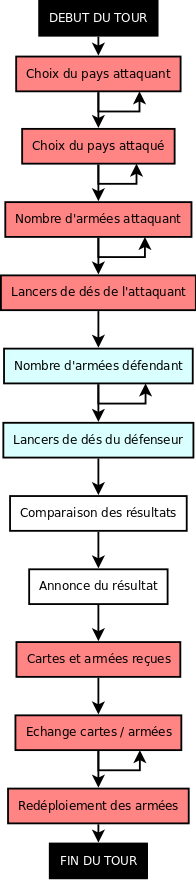
\includegraphics[width=5cm]{Images/tour_jeu.png}
    \caption{Déroulement d'un tour de jeu pour un joueur}
    \label{fig:tour de jeu}
\end{figure}


\newpage
\subsection{Conception logiciel}

\begin{landscape}
    \begin{figure}[!htbp]
        \centering
        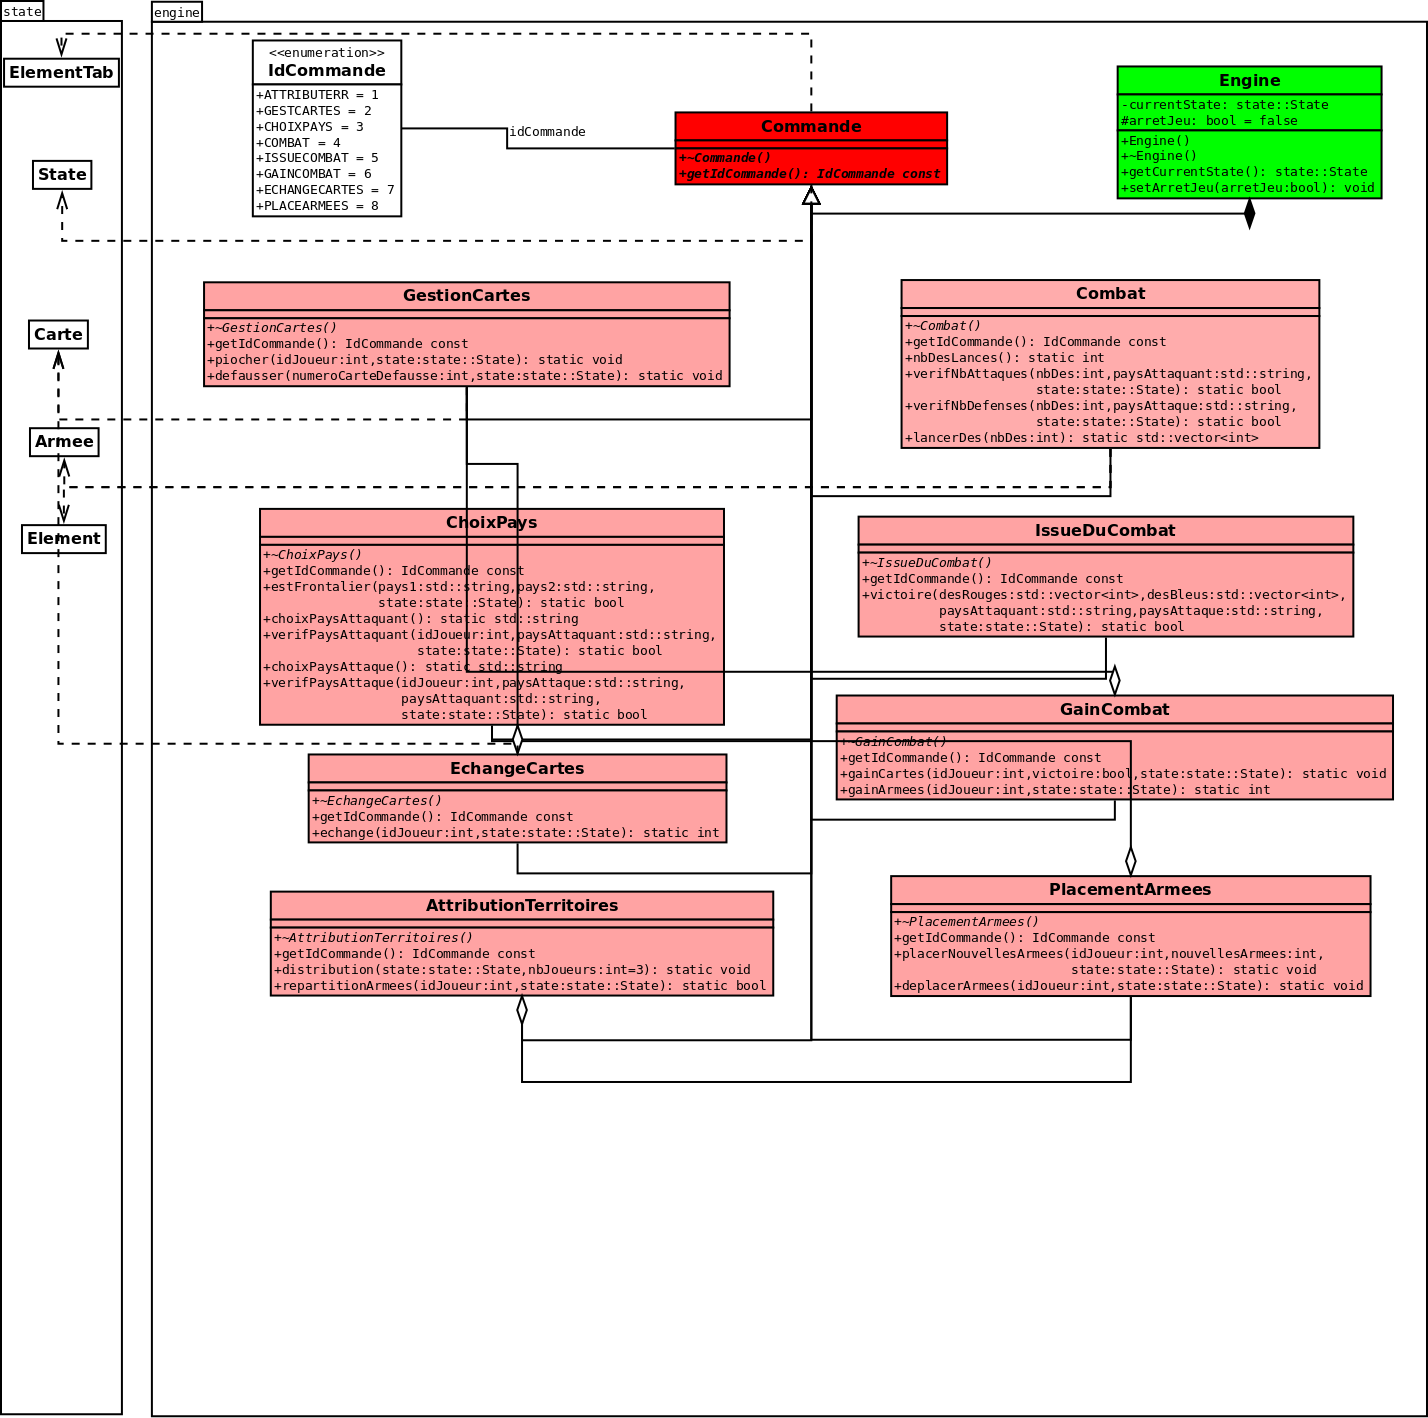
\includegraphics[width=21cm]{Images/engine.png}
        \caption{Diagramme du moteur du jeu}
        \label{fig:state}
    \end{figure}
\end{landscape}